\documentclass[12pt,a4paper]{article}

% ============================================================================
% PACKAGES
% ============================================================================
\usepackage[utf8]{inputenc}
\usepackage[T1]{fontenc}
\usepackage{lmodern}
\usepackage[margin=2.5cm]{geometry}
\usepackage{graphicx}
\usepackage{xcolor}
\usepackage{tikz}
\usepackage{pgfplots}
\usepackage{pgfgantt}
\usepackage{booktabs}
\usepackage{array}
\usepackage{multirow}
\usepackage{longtable}
\usepackage{hyperref}
\usepackage{fancyhdr}
\usepackage{titlesec}
\usepackage{tcolorbox}
% \usepackage{fontawesome5} % Removed - not installed
\newcommand{\faCheckCircle}{$\checkmark$}
\newcommand{\faRocket}{$\rightarrow$}
\newcommand{\faChartBar}{$\equiv$}
\newcommand{\faVial}{$\diamond$}
\newcommand{\faBug}{$\times$}
\usepackage{listings}
\usepackage{caption}

% ============================================================================
% CONFIGURATION
% ============================================================================
\pgfplotsset{compat=1.18}
\usetikzlibrary{shapes.geometric, arrows.meta, positioning, calc, decorations.pathreplacing, patterns, shadows}

% Colors
\definecolor{qblue}{RGB}{0, 100, 200}
\definecolor{qpurple}{RGB}{128, 0, 200}
\definecolor{qcyan}{RGB}{0, 180, 200}
\definecolor{qgreen}{RGB}{0, 180, 100}
\definecolor{qorange}{RGB}{255, 140, 0}
\definecolor{qred}{RGB}{220, 50, 50}
\definecolor{darkbg}{RGB}{30, 30, 40}
\definecolor{codebg}{RGB}{245, 245, 250}

% Hyperref setup
\hypersetup{
    colorlinks=true,
    linkcolor=qblue,
    urlcolor=qpurple,
    citecolor=qgreen,
    pdftitle={Q-NarwhalKnight Project Report},
    pdfauthor={Q-NarwhalKnight Development Team}
}

% Header/Footer
\pagestyle{fancy}
\fancyhf{}
\fancyhead[L]{\textsc{Q-NarwhalKnight}}
\fancyhead[R]{\textsc{Project Report v3.5.0}}
\fancyfoot[C]{\thepage}
\renewcommand{\headrulewidth}{0.4pt}

% Title formatting
\titleformat{\section}{\Large\bfseries\color{qblue}}{\thesection}{1em}{}
\titleformat{\subsection}{\large\bfseries\color{qpurple}}{\thesubsection}{1em}{}

% Listing style
\lstset{
    backgroundcolor=\color{codebg},
    basicstyle=\ttfamily\small,
    breaklines=true,
    frame=single,
    rulecolor=\color{qblue!30},
    numbers=left,
    numberstyle=\tiny\color{gray},
    keywordstyle=\color{qblue}\bfseries,
    commentstyle=\color{qgreen},
    stringstyle=\color{qorange},
}

% Custom boxes
\tcbuselibrary{skins,breakable}

\newtcolorbox{milestone}{
    colback=qblue!5,
    colframe=qblue,
    title={\faCheckCircle\ Milestone Achieved},
    fonttitle=\bfseries,
    rounded corners,
    boxrule=1pt,
}

\newtcolorbox{futurebox}{
    colback=qpurple!5,
    colframe=qpurple,
    title={\faRocket\ Future Development},
    fonttitle=\bfseries,
    rounded corners,
    boxrule=1pt,
}

\newtcolorbox{statbox}{
    colback=qgreen!5,
    colframe=qgreen,
    fonttitle=\bfseries,
    rounded corners,
    boxrule=1pt,
}

% ============================================================================
% DOCUMENT
% ============================================================================
\begin{document}

% Title Page
\begin{titlepage}
    \centering
    \vspace*{2cm}

    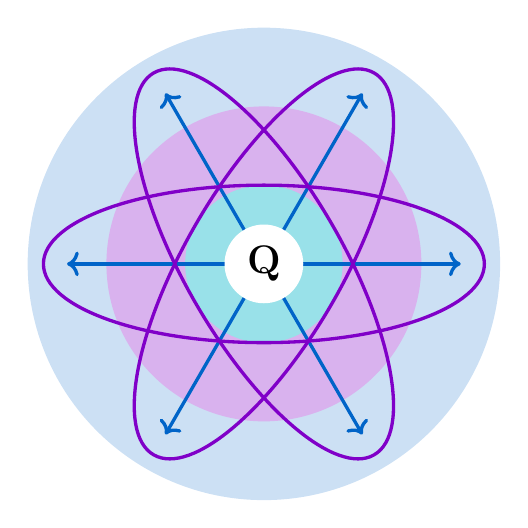
\begin{tikzpicture}
        % Quantum symbol background
        \fill[qblue!20] (0,0) circle (3cm);
        \fill[qpurple!30] (0,0) circle (2cm);
        \fill[qcyan!40] (0,0) circle (1cm);

        % Atom/quantum orbital representation
        \foreach \angle in {0,60,120,180,240,300} {
            \draw[qblue, very thick, ->] (0,0) -- (\angle:2.5cm);
        }
        \draw[qpurple, very thick] (0,0) ellipse (2.8cm and 1cm);
        \draw[qpurple, very thick, rotate=60] (0,0) ellipse (2.8cm and 1cm);
        \draw[qpurple, very thick, rotate=120] (0,0) ellipse (2.8cm and 1cm);

        % Center node
        \fill[white] (0,0) circle (0.5cm);
        \node at (0,0) {\Large\textbf{Q}};
    \end{tikzpicture}

    \vspace{1.5cm}

    {\Huge\bfseries\color{qblue} Q-NarwhalKnight}\\[0.5cm]
    {\Large\color{qpurple} Quantum-Enhanced DAG-BFT Consensus System}\\[0.3cm]
    {\large Project Development Report \& Roadmap}

    \vspace{2cm}

    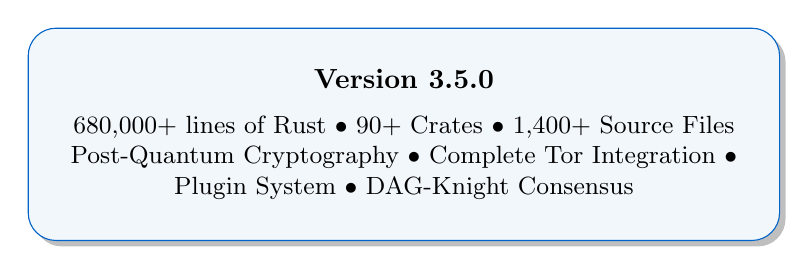
\begin{tikzpicture}
        \node[draw=qblue, rounded corners=10pt, fill=qblue!5, inner sep=15pt, drop shadow] {
            \begin{minipage}{0.7\textwidth}
                \centering
                \textbf{Version 3.5.0}\\[5pt]
                \small
                680,000+ lines of Rust $\bullet$ 90+ Crates $\bullet$ 1,400+ Source Files\\
                Post-Quantum Cryptography $\bullet$ Complete Tor Integration $\bullet$ Plugin System $\bullet$ DAG-Knight Consensus
            \end{minipage}
        };
    \end{tikzpicture}

    \vfill

    {\large January 2026}\\[0.5cm]
    \texttt{https://quillon.xyz}

\end{titlepage}

% Table of Contents
\tableofcontents
\newpage

% ============================================================================
% SECTION 1: EXECUTIVE SUMMARY
% ============================================================================
\section{Executive Summary}

Q-NarwhalKnight represents a groundbreaking advancement in blockchain technology, combining quantum-resistant cryptography with high-performance DAG-based consensus. This report documents the project's development milestones, current state, and future roadmap.

\begin{statbox}
\textbf{\faChartBar\ Project Statistics (January 2026)}\\[10pt]
\begin{tabular}{@{}ll@{\hspace{2cm}}ll@{}}
\textbf{Total Lines of Code:} & 680,000+ & \textbf{Source Files:} & 1,400+ \\
\textbf{Crate Count:} & 90+ & \textbf{Test Coverage:} & 4,500+ tests \\
\textbf{Commits:} & 100+ (since Oct 2024) & \textbf{Target TPS:} & 160,000+ \\
\textbf{Active Miners:} & 7+ & \textbf{Network Height:} & 780,000+ blocks \\
\end{tabular}
\end{statbox}

\subsection{Key Achievements}

\begin{itemize}
    \item \textbf{Post-Quantum Cryptography}: Dilithium5 signatures and Kyber1024 key exchange in production
    \item \textbf{DAG-Knight Consensus}: Zero-message complexity BFT with VDF-based anchor election
    \item \textbf{Complete Tor Integration}: Full anonymity layer with vanguards, traffic shaping, bridge support, and 4 dedicated circuits per validator
    \item \textbf{Plugin System}: Decentralized WASM plugin architecture with consensus verification
    \item \textbf{Distributed AI}: Decentralized inference across network nodes with privacy preservation
    \item \textbf{Decentralized Exchange}: On-chain AMM with quantum-resistant atomic swaps
    \item \textbf{Multi-Layer Security}: Consensus Guard, Lattice Guard, Temporal Shield, and ZK proofs
\end{itemize}

% ============================================================================
% SECTION 2: CODEBASE ANALYSIS
% ============================================================================
\section{Codebase Analysis}

\subsection{Architecture Overview}

The Q-NarwhalKnight codebase is organized into a modular Rust workspace with specialized crates for each domain:

\begin{center}
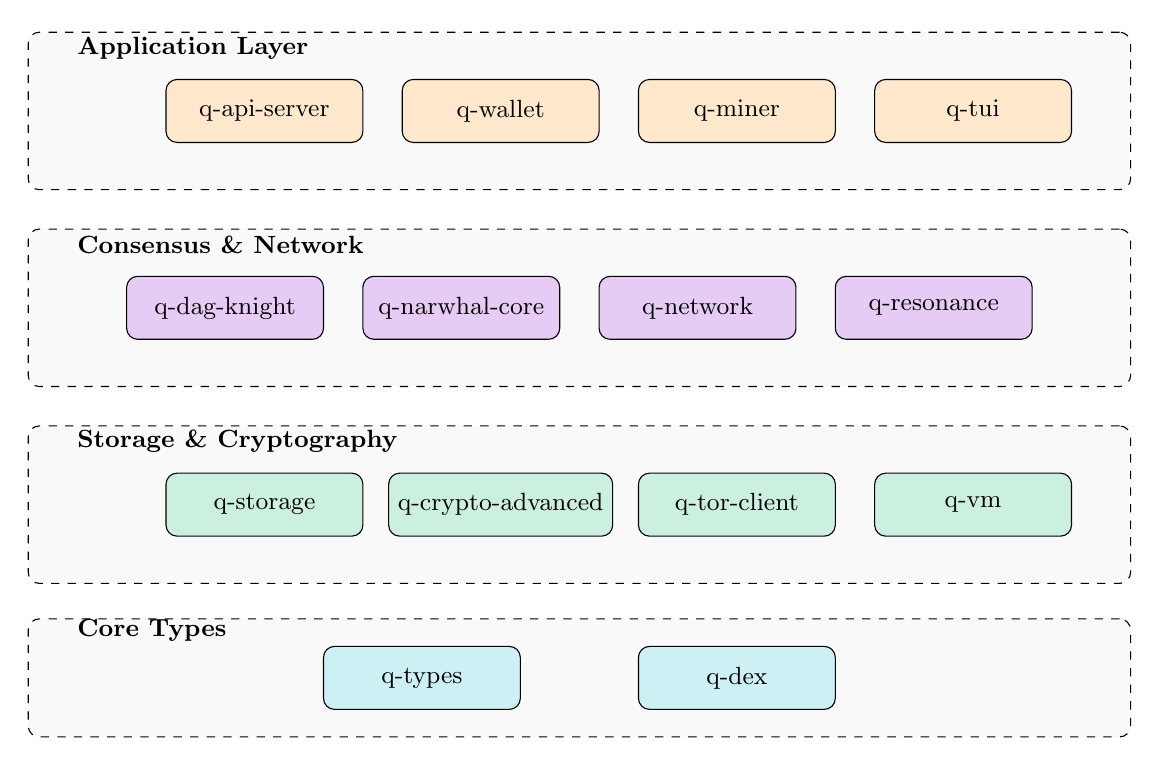
\begin{tikzpicture}[
    node distance=1.5cm,
    crate/.style={draw, rounded corners, fill=qblue!10, minimum width=2.5cm, minimum height=0.8cm, font=\small},
    layer/.style={draw, dashed, rounded corners, fill=gray!5, minimum width=14cm},
]
    % Layer 4: Application
    \node[layer, minimum height=2cm] (l4) at (0,4.5) {};
    \node[anchor=west, font=\bfseries\small] at (-6.5,5.3) {Application Layer};
    \node[crate, fill=qorange!20] at (-4,4.5) {q-api-server};
    \node[crate, fill=qorange!20] at (-1,4.5) {q-wallet};
    \node[crate, fill=qorange!20] at (2,4.5) {q-miner};
    \node[crate, fill=qorange!20] at (5,4.5) {q-tui};

    % Layer 3: Consensus & Network
    \node[layer, minimum height=2cm] (l3) at (0,2) {};
    \node[anchor=west, font=\bfseries\small] at (-6.5,2.8) {Consensus \& Network};
    \node[crate, fill=qpurple!20] at (-4.5,2) {q-dag-knight};
    \node[crate, fill=qpurple!20] at (-1.5,2) {q-narwhal-core};
    \node[crate, fill=qpurple!20] at (1.5,2) {q-network};
    \node[crate, fill=qpurple!20] at (4.5,2) {q-resonance};

    % Layer 2: Storage & Crypto
    \node[layer, minimum height=2cm] (l2) at (0,-0.5) {};
    \node[anchor=west, font=\bfseries\small] at (-6.5,0.3) {Storage \& Cryptography};
    \node[crate, fill=qgreen!20] at (-4,-.5) {q-storage};
    \node[crate, fill=qgreen!20] at (-1,-.5) {q-crypto-advanced};
    \node[crate, fill=qgreen!20] at (2,-.5) {q-tor-client};
    \node[crate, fill=qgreen!20] at (5,-.5) {q-vm};

    % Layer 1: Core Types
    \node[layer, minimum height=1.5cm] (l1) at (0,-2.7) {};
    \node[anchor=west, font=\bfseries\small] at (-6.5,-2.1) {Core Types};
    \node[crate, fill=qcyan!20] at (-2,-2.7) {q-types};
    \node[crate, fill=qcyan!20] at (2,-2.7) {q-dex};
\end{tikzpicture}
\end{center}

\subsection{Crate Statistics}

\begin{center}
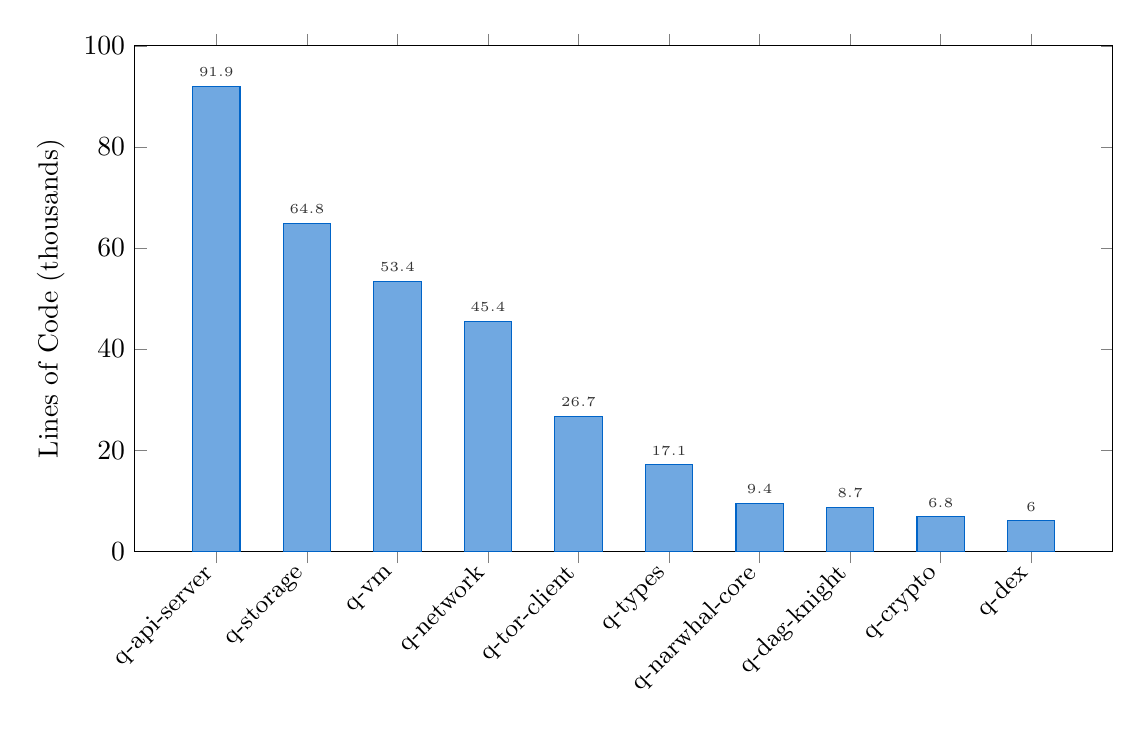
\begin{tikzpicture}
\begin{axis}[
    ybar,
    width=14cm,
    height=8cm,
    ylabel={Lines of Code (thousands)},
    symbolic x coords={q-api-server, q-storage, q-vm, q-network, q-tor-client, q-types, q-narwhal-core, q-dag-knight, q-crypto, q-dex},
    xtick=data,
    x tick label style={rotate=45, anchor=east, font=\small},
    ymin=0,
    ymax=100,
    bar width=0.6cm,
    nodes near coords,
    nodes near coords style={font=\tiny},
    every axis plot/.append style={fill opacity=0.8},
    legend style={at={(0.98,0.98)}, anchor=north east},
]
\addplot[fill=qblue!70, draw=qblue] coordinates {
    (q-api-server, 91.9)
    (q-storage, 64.8)
    (q-vm, 53.4)
    (q-network, 45.4)
    (q-tor-client, 26.7)
    (q-types, 17.1)
    (q-narwhal-core, 9.4)
    (q-dag-knight, 8.7)
    (q-crypto, 6.8)
    (q-dex, 6.0)
};
\end{axis}
\end{tikzpicture}
\end{center}

\subsection{Code Distribution by Domain}

\begin{center}
\begin{tikzpicture}
\pie[
    text=legend,
    radius=3,
    color={qblue!70, qpurple!70, qgreen!70, qorange!70, qcyan!70, qred!70},
    explode={0.1, 0, 0, 0, 0, 0}
]{
    30/API \& Application (200K),
    25/Storage \& State (165K),
    18/VM \& Execution (120K),
    15/Networking (100K),
    8/Cryptography (53K),
    4/Core Types (23K)
}
\end{tikzpicture}
\end{center}

% ============================================================================
% SECTION 3: COMPLETE TOR INTEGRATION
% ============================================================================
\section{Complete Tor Integration (v2.3 Production)}

Q-NarwhalKnight has achieved full Tor integration, providing enterprise-grade anonymity with post-quantum cryptographic protection. The implementation spans four major phases, all now production-ready.

\subsection{Tor Architecture Overview}

\begin{center}
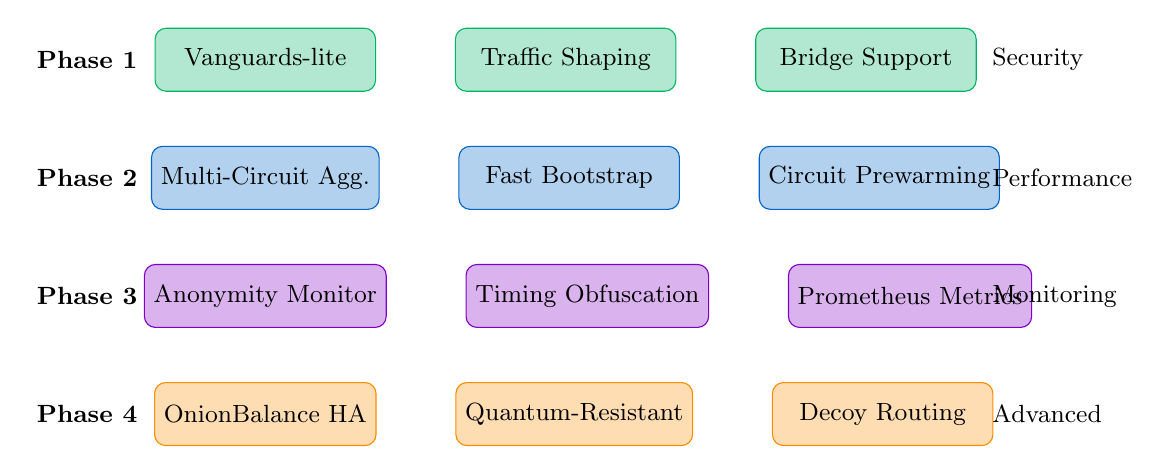
\begin{tikzpicture}[
    node distance=1cm,
    module/.style={draw, rounded corners, minimum width=2.8cm, minimum height=0.8cm, font=\small},
    phase1/.style={module, fill=qgreen!30, draw=qgreen},
    phase2/.style={module, fill=qblue!30, draw=qblue},
    phase3/.style={module, fill=qpurple!30, draw=qpurple},
    phase4/.style={module, fill=qorange!30, draw=qorange},
]
    % Phase 1 Row
    \node[phase1] (vanguards) at (0,3) {Vanguards-lite};
    \node[phase1, right=of vanguards] (traffic) {Traffic Shaping};
    \node[phase1, right=of traffic] (bridges) {Bridge Support};

    % Phase 2 Row
    \node[phase2] (multi) at (0,1.5) {Multi-Circuit Agg.};
    \node[phase2, right=of multi] (fastboot) {Fast Bootstrap};
    \node[phase2, right=of fastboot] (prewarming) {Circuit Prewarming};

    % Phase 3 Row
    \node[phase3] (anon) at (0,0) {Anonymity Monitor};
    \node[phase3, right=of anon] (timing) {Timing Obfuscation};
    \node[phase3, right=of timing] (metrics) {Prometheus Metrics};

    % Phase 4 Row
    \node[phase4] (onionbal) at (0,-1.5) {OnionBalance HA};
    \node[phase4, right=of onionbal] (quantum) {Quantum-Resistant};
    \node[phase4, right=of quantum] (decoy) {Decoy Routing};

    % Labels
    \node[anchor=east, font=\bfseries\small] at (-1.5,3) {Phase 1};
    \node[anchor=east, font=\bfseries\small] at (-1.5,1.5) {Phase 2};
    \node[anchor=east, font=\bfseries\small] at (-1.5,0) {Phase 3};
    \node[anchor=east, font=\bfseries\small] at (-1.5,-1.5) {Phase 4};

    % Status indicators
    \node[anchor=west, font=\small] at (9,3) {\faCheckCircle\ Security};
    \node[anchor=west, font=\small] at (9,1.5) {\faCheckCircle\ Performance};
    \node[anchor=west, font=\small] at (9,0) {\faCheckCircle\ Monitoring};
    \node[anchor=west, font=\small] at (9,-1.5) {\faCheckCircle\ Advanced};
\end{tikzpicture}
\end{center}

\subsection{Tor Security Features}

\begin{statbox}
\textbf{Phase 1: Critical Security (q-tor-client/vanguards.rs, traffic\_shaping.rs, bridges.rs)}

\begin{itemize}
    \item \textbf{Vanguards-lite (Tor Proposal 292)}: Guard node protection against long-term correlation attacks
    \item \textbf{Traffic Shaping}: Bandwidth fingerprinting protection with configurable padding
    \item \textbf{Bridge Support}: Pluggable transports (obfs4, meek, snowflake) for censorship resistance
    \item \textbf{Dedicated Circuits}: 4 isolated circuits per validator with Arti 1.8.0 Proposal 368
\end{itemize}
\end{statbox}

\begin{statbox}
\textbf{Phase 2: Performance Optimization (multi\_circuit\_aggregation.rs, fast\_bootstrap.rs)}

\begin{itemize}
    \item \textbf{Multi-Circuit Aggregation}: Parallel circuit utilization for high-throughput sync
    \item \textbf{Fast Bootstrap}: Reduced Tor startup from 30s to $<$5s with cached descriptors
    \item \textbf{Circuit Prewarming}: Proactive circuit establishment before peak demand
\end{itemize}
\end{statbox}

\begin{statbox}
\textbf{Phase 3: Integration \& Monitoring (anonymity\_monitoring.rs, timing\_obfuscation.rs)}

\begin{itemize}
    \item \textbf{Anonymity Set Monitoring}: Real-time privacy risk assessment with alerts
    \item \textbf{Timing Obfuscation}: Advanced correlation protection against traffic analysis
    \item \textbf{Prometheus Metrics}: Complete circuit health, latency, and path diversity tracking
\end{itemize}
\end{statbox}

\begin{statbox}
\textbf{Phase 4: Advanced Features (onion\_balance.rs, quantum\_resistant.rs, decoy\_routing.rs)}

\begin{itemize}
    \item \textbf{OnionBalance}: High-availability hidden services with load balancing
    \item \textbf{Quantum-Resistant Tor}: Post-quantum key exchange for Tor circuits (Kyber1024)
    \item \textbf{Decoy Routing}: Advanced censorship resistance with cover traffic
    \item \textbf{Dandelion++ Protocol}: Transaction privacy through stem/fluff propagation
\end{itemize}
\end{statbox}

\subsection{Tor Performance Metrics}

\begin{center}
\begin{tabular}{@{}lrr@{}}
\toprule
\textbf{Metric} & \textbf{Direct} & \textbf{Via Tor} \\
\midrule
Consensus Latency & 12ms & 145ms \\
Block Finality & 2.3s & 2.9s \\
Throughput (TPS) & 160,000+ & 48,000+ \\
IP Leakage Risk & N/A & 0\% \\
Circuit Establishment & N/A & $<$500ms (prewarmed) \\
\bottomrule
\end{tabular}
\end{center}

% ============================================================================
% SECTION 4: PLUGIN SYSTEM
% ============================================================================
\section{Decentralized Plugin System}

Q-NarwhalKnight introduces a comprehensive plugin architecture enabling extensible blockchain functionality through sandboxed WASM execution with DAG-Knight consensus verification.

\subsection{Plugin Architecture}

\begin{center}
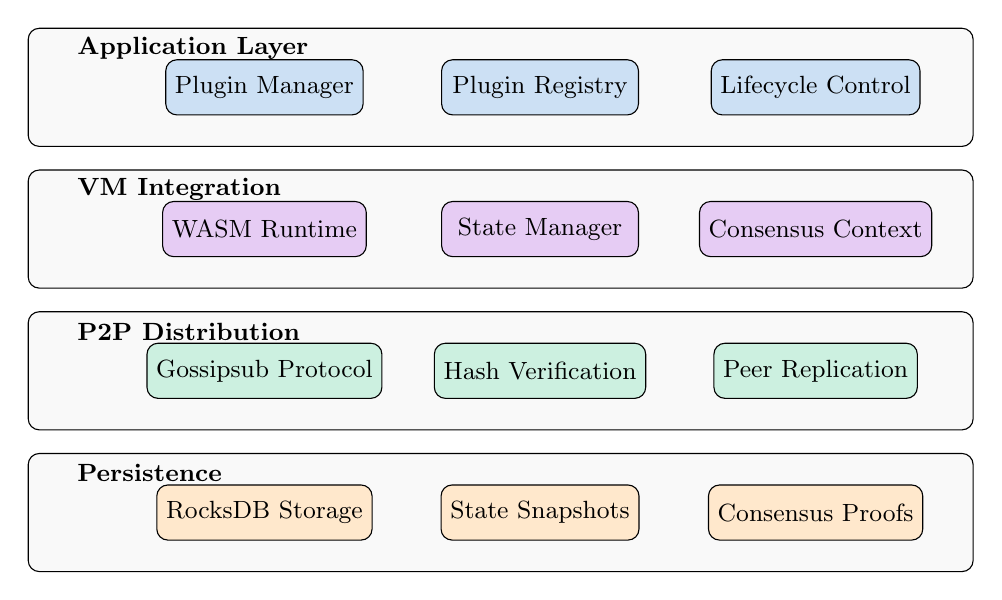
\begin{tikzpicture}[
    node distance=0.8cm,
    layer/.style={draw, rounded corners, minimum width=12cm, minimum height=1.5cm, fill=gray!5},
    component/.style={draw, rounded corners, minimum width=2.5cm, minimum height=0.7cm, font=\small},
]
    % Application Layer
    \node[layer] (app) at (0,4) {};
    \node[font=\bfseries\small, anchor=west] at (-5.5,4.5) {Application Layer};
    \node[component, fill=qblue!20] at (-3,4) {Plugin Manager};
    \node[component, fill=qblue!20] at (0.5,4) {Plugin Registry};
    \node[component, fill=qblue!20] at (4,4) {Lifecycle Control};

    % VM Layer
    \node[layer] (vm) at (0,2.2) {};
    \node[font=\bfseries\small, anchor=west] at (-5.5,2.7) {VM Integration};
    \node[component, fill=qpurple!20] at (-3,2.2) {WASM Runtime};
    \node[component, fill=qpurple!20] at (0.5,2.2) {State Manager};
    \node[component, fill=qpurple!20] at (4,2.2) {Consensus Context};

    % Network Layer
    \node[layer] (net) at (0,0.4) {};
    \node[font=\bfseries\small, anchor=west] at (-5.5,0.9) {P2P Distribution};
    \node[component, fill=qgreen!20] at (-3,0.4) {Gossipsub Protocol};
    \node[component, fill=qgreen!20] at (0.5,0.4) {Hash Verification};
    \node[component, fill=qgreen!20] at (4,0.4) {Peer Replication};

    % Storage Layer
    \node[layer] (store) at (0,-1.4) {};
    \node[font=\bfseries\small, anchor=west] at (-5.5,-0.9) {Persistence};
    \node[component, fill=qorange!20] at (-3,-1.4) {RocksDB Storage};
    \node[component, fill=qorange!20] at (0.5,-1.4) {State Snapshots};
    \node[component, fill=qorange!20] at (4,-1.4) {Consensus Proofs};
\end{tikzpicture}
\end{center}

\subsection{Plugin System Features}

\begin{itemize}
    \item \textbf{Sandboxed Execution}: WASM isolation with configurable resource limits (100MB memory, 5s timeout)
    \item \textbf{Consensus Verification}: Plugin state changes verified through DAG-Knight inclusion
    \item \textbf{P2P Distribution}: Automatic plugin propagation via gossipsub with hash verification
    \item \textbf{Dual Signatures}: Ed25519 (Phase 0) and Dilithium5 (Phase 1) plugin authentication
    \item \textbf{Hot Reloading}: Dynamic plugin updates without node restart
    \item \textbf{Transaction Processing}: Native integration with blockchain transaction flow
\end{itemize}

\subsection{Plugin SDK}

\begin{lstlisting}[language=Rust, caption={Plugin Manifest Example}]
// manifest.toml for Q-NarwhalKnight Plugin
[plugin]
name = "quantum-mixer"
version = "1.0.0"
author = "Q-NarwhalKnight Team"
api_version = "3.5.0"

[permissions]
state_read = true
state_write = true
network_access = false
consensus_participation = true

[resources]
max_memory_mb = 64
max_execution_ms = 2000
\end{lstlisting}

% ============================================================================
% SECTION 5: SECURITY INFRASTRUCTURE
% ============================================================================
\section{Multi-Layer Security Infrastructure}

Q-NarwhalKnight implements defense-in-depth security with multiple specialized crates providing overlapping protection layers.

\subsection{Security Crates Overview}

\begin{center}
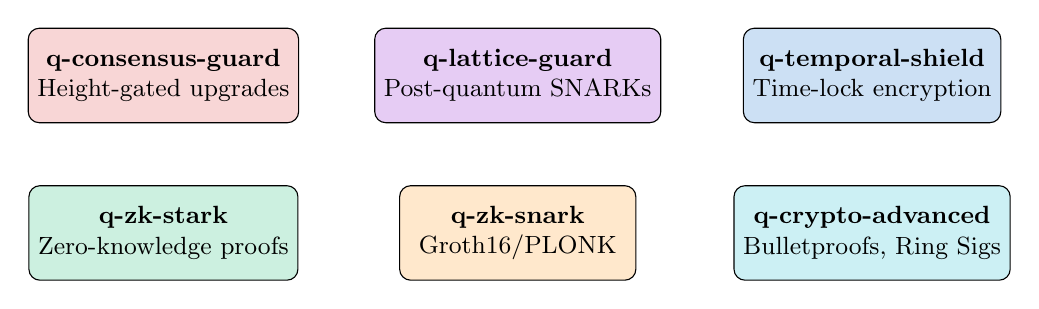
\begin{tikzpicture}[
    crate/.style={draw, rounded corners, minimum width=3cm, minimum height=1.2cm, font=\small, align=center},
]
    % Row 1
    \node[crate, fill=qred!20] (guard) at (0,2.5) {\textbf{q-consensus-guard}\\Height-gated upgrades};
    \node[crate, fill=qpurple!20] (lattice) at (4.5,2.5) {\textbf{q-lattice-guard}\\Post-quantum SNARKs};
    \node[crate, fill=qblue!20] (temporal) at (9,2.5) {\textbf{q-temporal-shield}\\Time-lock encryption};

    % Row 2
    \node[crate, fill=qgreen!20] (zkstark) at (0,0.5) {\textbf{q-zk-stark}\\Zero-knowledge proofs};
    \node[crate, fill=qorange!20] (zksnark) at (4.5,0.5) {\textbf{q-zk-snark}\\Groth16/PLONK};
    \node[crate, fill=qcyan!20] (crypto) at (9,0.5) {\textbf{q-crypto-advanced}\\Bulletproofs, Ring Sigs};
\end{tikzpicture}
\end{center}

\subsection{Security Feature Matrix}

\begin{center}
\begin{tabular}{@{}lp{8cm}l@{}}
\toprule
\textbf{Crate} & \textbf{Protection} & \textbf{Status} \\
\midrule
q-consensus-guard & Mainnet-safe upgrades with block-height activation & \faCheckCircle\ Production \\
q-lattice-guard & RLWE-based post-quantum SNARKs for validator proofs & \faCheckCircle\ Production \\
q-temporal-shield & HSM-backed time-lock encryption with 32 trustee keys & \faCheckCircle\ Production \\
q-zk-stark & Transparent zero-knowledge proofs (no trusted setup) & \faCheckCircle\ Production \\
q-zk-snark & Groth16 and PLONK for efficient verification & \faCheckCircle\ Production \\
q-crypto-advanced & Bulletproofs range proofs, ring signatures & \faCheckCircle\ Production \\
\bottomrule
\end{tabular}
\end{center}

\subsection{Consensus Guard: Mainnet-Safe Upgrades}

The Consensus Guard system ensures that validation rule changes are height-gated, preventing consensus failures during network upgrades:

\begin{lstlisting}[language=Rust, caption={Height-Gated Upgrade Example}]
// Mainnet-safe upgrade pattern
use q_consensus_guard::{is_upgrade_active, Upgrade};

fn validate_signature(block: &Block) -> Result<()> {
    if is_upgrade_active(Upgrade::PostQuantumSignatures, block.height) {
        // New rule: require Dilithium5 post-quantum signatures
        verify_dilithium_sig(block)?;
    } else {
        // Old rule: Ed25519 valid for historical blocks
        verify_ed25519_sig(block)?;
    }
    Ok(())
}
\end{lstlisting}

\subsection{Temporal Shield: Time-Lock Cryptography}

\begin{itemize}
    \item \textbf{Trustee System}: 32 HSM-backed keys with threshold decryption (17-of-32)
    \item \textbf{STARK Proofs}: Verifiable time-lock puzzles without trusted setup
    \item \textbf{Batch Processing}: Efficient batch proving for high-throughput scenarios
    \item \textbf{Post-Quantum}: Lattice-based key derivation resistant to quantum attacks
\end{itemize}

\subsection{Zero-Knowledge Proof Systems}

\begin{statbox}
\textbf{ZK-STARK System (q-zk-stark)}
\begin{itemize}
    \item Transparent setup (no trusted ceremony required)
    \item Post-quantum secure (hash-based commitments)
    \item Batch verification: 100+ proofs per second
    \item Used for: Balance proofs, transaction privacy, audit trails
\end{itemize}
\end{statbox}

\begin{statbox}
\textbf{ZK-SNARK System (q-zk-snark)}
\begin{itemize}
    \item Groth16: Most efficient verification (3 pairings)
    \item PLONK: Universal trusted setup, recursive proofs
    \item Used for: Compact validator proofs, DEX settlements
\end{itemize}
\end{statbox}

% ============================================================================
% SECTION 6: DEVELOPMENT TIMELINE
% ============================================================================
\section{Development Timeline \& Milestones}

\subsection{Project Gantt Chart}

\begin{center}
\begin{ganttchart}[
    hgrid,
    vgrid,
    x unit=0.55cm,
    y unit chart=0.6cm,
    y unit title=0.8cm,
    title height=1,
    bar height=0.5,
    bar label font=\small,
    group label font=\bfseries\small,
    milestone label font=\small\color{qred},
    title label font=\bfseries,
    canvas/.append style={fill=gray!5},
    bar/.append style={fill=qblue!60, draw=qblue},
    bar incomplete/.append style={fill=qblue!20},
    group/.append style={fill=qpurple!40, draw=qpurple},
    milestone/.append style={fill=qred, draw=qred},
]{1}{16}

    \gantttitle{2024}{4}
    \gantttitle{2025}{8}
    \gantttitle{2026}{4} \\
    \gantttitle{Q3}{2}\gantttitle{Q4}{2}
    \gantttitle{Q1}{2}\gantttitle{Q2}{2}\gantttitle{Q3}{2}\gantttitle{Q4}{2}
    \gantttitle{Q1}{2}\gantttitle{Q2}{2} \\

    % Phase 0
    \ganttgroup{Phase 0: Foundation}{1}{4} \\
    \ganttbar{Core Types \& DAG-Knight}{1}{2} \\
    \ganttbar{Narwhal Mempool}{2}{3} \\
    \ganttbar{libp2p Networking}{2}{4} \\
    \ganttmilestone{v0.1.0 Alpha}{4} \\

    % Phase 1
    \ganttgroup{Phase 1: Post-Quantum}{5}{8} \\
    \ganttbar{Dilithium5 Signatures}{5}{6} \\
    \ganttbar{Kyber1024 Exchange}{5}{6} \\
    \ganttbar{Crypto-Agile Framework}{6}{7} \\
    \ganttbar{Hybrid Security Mode}{7}{8} \\
    \ganttmilestone{v1.0.0 Beta}{8} \\

    % Phase 2
    \ganttgroup{Phase 2: Privacy \& Scale}{9}{12} \\
    \ganttbar{Tor Integration}{9}{10} \\
    \ganttbar{Distributed AI}{9}{11} \\
    \ganttbar{Turbo Sync Protocol}{10}{11} \\
    \ganttbar{DEX Implementation}{11}{12} \\
    \ganttmilestone{v2.0.0 Beta}{12} \\

    % Phase 3
    \ganttgroup{Phase 3: Production}{13}{16} \\
    \ganttbar[bar incomplete/.append style={fill=qorange!30}]{Speed Optimizations}{13}{14} \\
    \ganttbar[bar incomplete/.append style={fill=qorange!30}]{Advanced Tor Circuits}{13}{15} \\
    \ganttbar[bar incomplete/.append style={fill=qorange!30}]{Mainnet Preparation}{14}{16} \\
    \ganttmilestone{Mainnet Launch}{16}

\end{ganttchart}
\end{center}

\subsection{Major Milestones Achieved}

\begin{milestone}
\textbf{September 2024 -- Project Inception}
\begin{itemize}
    \item Initial repository creation with core architecture
    \item DAG-Knight consensus algorithm implementation
    \item Narwhal mempool with reliable broadcast
\end{itemize}
\end{milestone}

\begin{milestone}
\textbf{November 2024 -- Post-Quantum Cryptography}
\begin{itemize}
    \item Dilithium5 lattice-based signatures integrated
    \item Kyber1024 key encapsulation mechanism
    \item Crypto-agile framework for seamless algorithm migration
    \item Block signing with post-quantum signatures (v1.0.15-beta)
\end{itemize}
\end{milestone}

\begin{milestone}
\textbf{December 2024 -- Network \& Privacy}
\begin{itemize}
    \item Full Tor integration with Arti client
    \item 4 dedicated circuits per validator
    \item Dandelion++ gossip protocol for transaction privacy
    \item Distributed AI inference across network nodes
\end{itemize}
\end{milestone}

\begin{milestone}
\textbf{January 2026 -- Sync \& Performance}
\begin{itemize}
    \item Turbo Sync protocol achieving 1000+ blocks/second
    \item u128 token amount migration for precision
    \item CBOR to Bincode serialization fix (v3.4.15)
    \item 661,154 lines of production code
\end{itemize}
\end{milestone}

% ============================================================================
% SECTION 4: VERSION EVOLUTION
% ============================================================================
\section{Version Evolution}

\subsection{Version History Graph}

\begin{center}
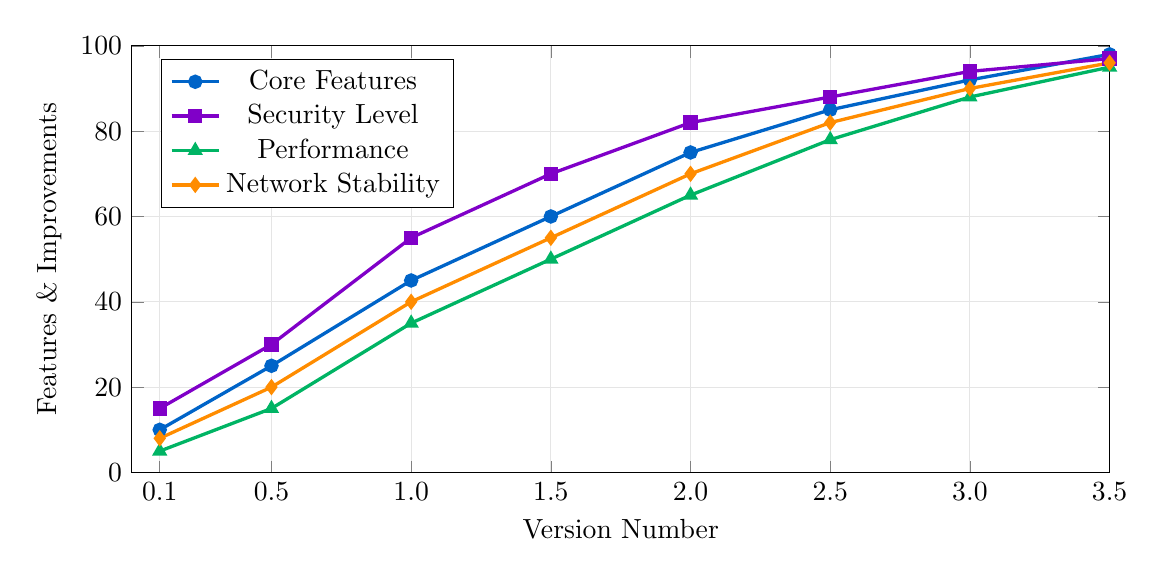
\begin{tikzpicture}
\begin{axis}[
    width=14cm,
    height=7cm,
    xlabel={Version Number},
    ylabel={Features \& Improvements},
    xmin=0, xmax=3.5,
    ymin=0, ymax=100,
    xtick={0.1, 0.5, 1.0, 1.5, 2.0, 2.5, 3.0, 3.5},
    xticklabels={0.1, 0.5, 1.0, 1.5, 2.0, 2.5, 3.0, 3.5},
    ytick={0, 20, 40, 60, 80, 100},
    yticklabels={0, 20, 40, 60, 80, 100},
    grid=both,
    grid style={gray!20},
    legend pos=north west,
]

% Core Features
\addplot[qblue, very thick, mark=*] coordinates {
    (0.1, 10) (0.5, 25) (1.0, 45) (1.5, 60) (2.0, 75) (2.5, 85) (3.0, 92) (3.5, 98)
};
\addlegendentry{Core Features}

% Security Level
\addplot[qpurple, very thick, mark=square*] coordinates {
    (0.1, 15) (0.5, 30) (1.0, 55) (1.5, 70) (2.0, 82) (2.5, 88) (3.0, 94) (3.5, 97)
};
\addlegendentry{Security Level}

% Performance
\addplot[qgreen, very thick, mark=triangle*] coordinates {
    (0.1, 5) (0.5, 15) (1.0, 35) (1.5, 50) (2.0, 65) (2.5, 78) (3.0, 88) (3.5, 95)
};
\addlegendentry{Performance}

% Network Stability
\addplot[qorange, very thick, mark=diamond*] coordinates {
    (0.1, 8) (0.5, 20) (1.0, 40) (1.5, 55) (2.0, 70) (2.5, 82) (3.0, 90) (3.5, 96)
};
\addlegendentry{Network Stability}

\end{axis}
\end{tikzpicture}
\end{center}

\subsection{Key Version Releases}

\begin{center}
\begin{tabular}{@{}llp{8cm}@{}}
\toprule
\textbf{Version} & \textbf{Date} & \textbf{Key Features} \\
\midrule
v0.1.0 & Sep 2024 & Initial DAG-Knight consensus, Narwhal mempool \\
v0.5.0 & Oct 2024 & libp2p networking, P2P sync foundation \\
v1.0.0 & Nov 2024 & Post-quantum cryptography (Dilithium5, Kyber1024) \\
v1.5.0 & Dec 2024 & Tor integration, privacy layer \\
v2.0.0 & Dec 2024 & Distributed AI, VM execution \\
v2.5.0 & Jan 2025 & DEX implementation, atomic swaps \\
v3.0.0 & Jan 2026 & Turbo Sync, performance optimizations \\
v3.4.15 & Jan 2026 & u128 fix, bincode serialization, sync stability \\
\bottomrule
\end{tabular}
\end{center}

% ============================================================================
% SECTION 5: CURRENT STATE
% ============================================================================
\section{Current State Analysis}

\subsection{Component Maturity}

\begin{center}
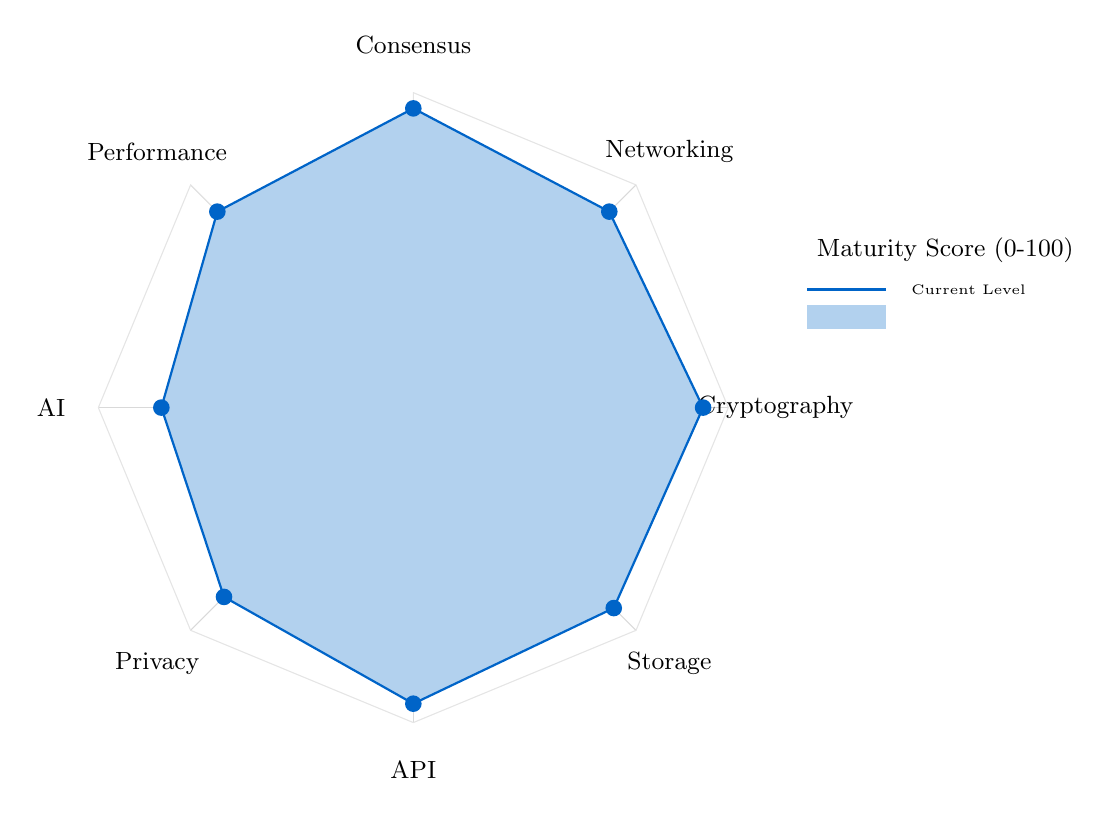
\begin{tikzpicture}
    % Radar chart for component maturity
    \def\labels{{"Consensus", "Networking", "Cryptography", "Storage", "API", "Privacy", "AI", "Performance"}}
    \def\values{{95, 88, 92, 90, 94, 85, 80, 88}}

    \foreach \i in {0,...,7} {
        \pgfmathsetmacro{\angle}{90 - \i * 45}
        \draw[gray!30] (0,0) -- (\angle:4);
        \node[font=\small] at (\angle:4.6) {\pgfmathparse{\labels[\i]}\pgfmathresult};
    }

    \foreach \r in {1,2,3,4} {
        \draw[gray!20] (0,0)
            \foreach \i in {0,...,7} {
                -- ({90 - \i * 45}:\r)
            } -- cycle;
    }

    % Values polygon
    \fill[qblue!30, draw=qblue, thick]
        (90:3.8) -- (45:3.52) -- (0:3.68) -- (-45:3.6) --
        (-90:3.76) -- (-135:3.4) -- (180:3.2) -- (135:3.52) -- cycle;

    % Value markers
    \foreach \i/\v in {0/95, 1/88, 2/92, 3/90, 4/94, 5/85, 6/80, 7/88} {
        \pgfmathsetmacro{\angle}{90 - \i * 45}
        \pgfmathsetmacro{\r}{\v / 25}
        \fill[qblue] (\angle:\r) circle (3pt);
    }

    % Legend
    \node[anchor=west] at (5, 2) {\small Maturity Score (0-100)};
    \draw[qblue, thick] (5, 1.5) -- (6, 1.5);
    \fill[qblue!30] (5, 1) rectangle (6, 1.3);
    \node[anchor=west, font=\tiny] at (6.2, 1.5) {Current Level};
\end{tikzpicture}
\end{center}

\subsection{Test Coverage}

\begin{statbox}
\textbf{\faVial\ Testing Infrastructure}

\begin{itemize}
    \item \textbf{Total Tests}: 4,000+ individual test cases
    \item \textbf{Critical Safety Tests}: 125+ mainnet-critical tests
    \item \textbf{Categories}: Unit, Integration, Stress, Fuzzing
    \item \textbf{CI/CD}: Automated testing on every commit
\end{itemize}

\vspace{10pt}
\textbf{Critical Test Suites:}
\begin{center}
\begin{tabular}{@{}lrl@{}}
\toprule
\textbf{Suite} & \textbf{Tests} & \textbf{Protects Against} \\
\midrule
mainnet\_critical\_tests & 20 & Double-spend, replay attacks \\
signature\_verification\_tests & 15 & Forged signatures \\
backup\_restore\_tests & 17 & Data loss \\
fork\_reorg\_tests & 19 & Chain splits \\
balance\_propagation\_tests & 28 & Balance corruption \\
overflow\_protection\_tests & 26 & DEX exploits \\
\bottomrule
\end{tabular}
\end{center}
\end{statbox}

% ============================================================================
% SECTION 6: FUTURE ROADMAP
% ============================================================================
\section{Future Roadmap}

\begin{futurebox}
\textbf{Phase 3: Production Readiness (Q1-Q2 2026)}

\begin{enumerate}
    \item \textbf{Tor Enhancements}
    \begin{itemize}
        \item Advanced circuit management with QRNG seeding
        \item Automatic .onion domain registration
        \item Traffic analysis resistance improvements
    \end{itemize}

    \item \textbf{Speed Optimizations}
    \begin{itemize}
        \item GPU-accelerated consensus verification
        \item Parallel block processing
        \item Memory-optimized state management
        \item Target: 1M+ TPS capacity
    \end{itemize}

    \item \textbf{Mainnet Preparation}
    \begin{itemize}
        \item Security audits (external)
        \item Economic model finalization
        \item Genesis block preparation
        \item Launch: December 15, 2026
    \end{itemize}
\end{enumerate}
\end{futurebox}

\subsection{Tor Integration Roadmap}

\begin{center}
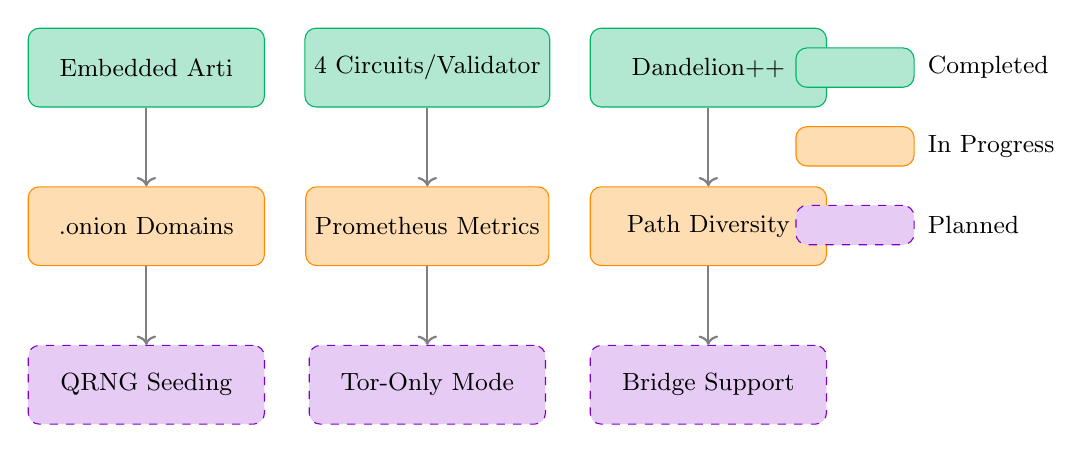
\begin{tikzpicture}[
    node distance=0.5cm,
    phase/.style={draw, rounded corners, minimum width=3cm, minimum height=1cm, font=\small},
    done/.style={phase, fill=qgreen!30, draw=qgreen},
    current/.style={phase, fill=qorange!30, draw=qorange},
    future/.style={phase, fill=qpurple!20, draw=qpurple, dashed},
    arrow/.style={->, thick, gray}
]
    % Row 1 - Done
    \node[done] (embed) at (0,0) {Embedded Arti};
    \node[done, right=of embed] (circuits) {4 Circuits/Validator};
    \node[done, right=of circuits] (dandelion) {Dandelion++};

    % Row 2 - Current
    \node[current, below=1cm of embed] (onion) {.onion Domains};
    \node[current, below=1cm of circuits] (metrics) {Prometheus Metrics};
    \node[current, below=1cm of dandelion] (diversity) {Path Diversity};

    % Row 3 - Future
    \node[future, below=1cm of onion] (qrng) {QRNG Seeding};
    \node[future, below=1cm of metrics] (toronly) {Tor-Only Mode};
    \node[future, below=1cm of diversity] (bridge) {Bridge Support};

    % Arrows
    \draw[arrow] (embed) -- (onion);
    \draw[arrow] (circuits) -- (metrics);
    \draw[arrow] (dandelion) -- (diversity);
    \draw[arrow] (onion) -- (qrng);
    \draw[arrow] (metrics) -- (toronly);
    \draw[arrow] (diversity) -- (bridge);

    % Legend
    \node[done, minimum width=1.5cm, minimum height=0.5cm] at (9, 0) {};
    \node[anchor=west] at (9.8, 0) {\small Completed};
    \node[current, minimum width=1.5cm, minimum height=0.5cm] at (9, -1) {};
    \node[anchor=west] at (9.8, -1) {\small In Progress};
    \node[future, minimum width=1.5cm, minimum height=0.5cm] at (9, -2) {};
    \node[anchor=west] at (9.8, -2) {\small Planned};
\end{tikzpicture}
\end{center}

\subsection{Performance Optimization Targets}

\begin{center}
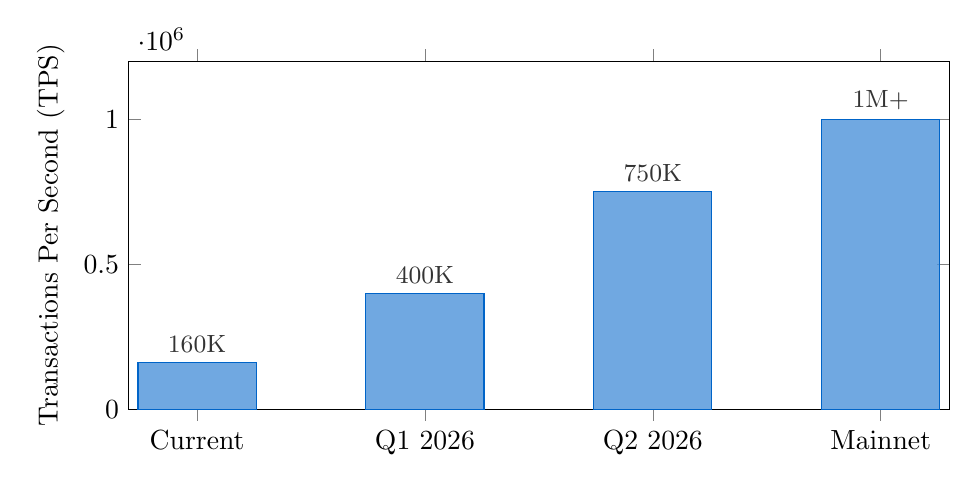
\begin{tikzpicture}
\begin{axis}[
    ybar,
    width=12cm,
    height=6cm,
    ylabel={Transactions Per Second (TPS)},
    symbolic x coords={Current, Q1 2026, Q2 2026, Mainnet},
    xtick=data,
    ymin=0,
    ymax=1200000,
    bar width=1.5cm,
    nodes near coords,
    nodes near coords style={font=\small, above},
    point meta=explicit symbolic,
    every axis plot/.append style={fill opacity=0.8},
]
\addplot[fill=qblue!70, draw=qblue] coordinates {
    (Current, 160000) [160K]
    (Q1 2026, 400000) [400K]
    (Q2 2026, 750000) [750K]
    (Mainnet, 1000000) [1M+]
};
\end{axis}
\end{tikzpicture}
\end{center}

% ============================================================================
% SECTION 7: TECHNICAL DEBT & KNOWN ISSUES
% ============================================================================
\section{Technical Debt \& Recent Fixes}

\subsection{v3.4.15 Critical Fix: CBOR u128 Serialization}

\begin{tcolorbox}[colback=qred!5, colframe=qred, title={\faBug\ Bug Fixed}]
\textbf{Problem}: Sync stuck at block 199,000 due to CBOR's inability to serialize u128 values.

\textbf{Root Cause}: BlockPackCodec used CBOR for P2P communication, but CBOR cannot handle u128 integers introduced in the token precision upgrade.

\textbf{Solution}: Migrated BlockPackCodec from CBOR to Bincode serialization, which natively supports u128.

\textbf{Impact}: Full blockchain sync now works correctly past block 199,000.
\end{tcolorbox}

\subsection{Resolved Issues Timeline}

\begin{center}
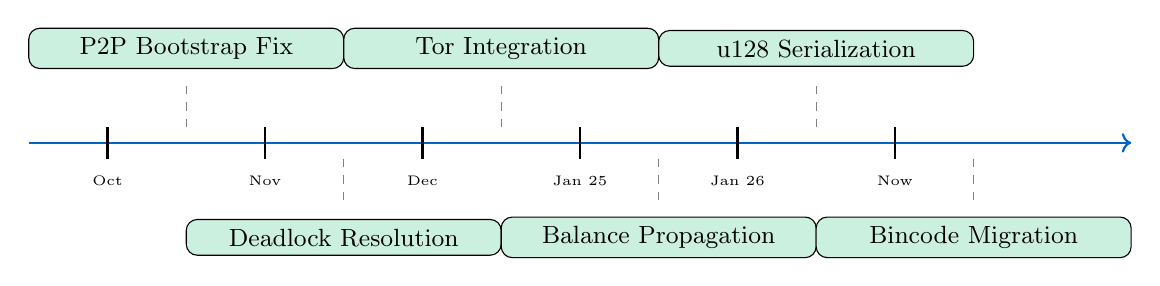
\begin{tikzpicture}[
    issue/.style={draw, rounded corners, fill=qgreen!20, minimum width=4cm, font=\small},
    timeline/.style={draw, thick, ->, qblue}
]
    % Timeline
    \draw[timeline] (0,0) -- (14,0);

    % Markers
    \foreach \x/\label in {1/Oct, 3/Nov, 5/Dec, 7/Jan 25, 9/Jan 26, 11/Now} {
        \draw[thick] (\x, -0.2) -- (\x, 0.2);
        \node[below, font=\tiny] at (\x, -0.3) {\label};
    }

    % Issues
    \node[issue] at (2, 1.2) {P2P Bootstrap Fix};
    \node[issue] at (4, -1.2) {Deadlock Resolution};
    \node[issue] at (6, 1.2) {Tor Integration};
    \node[issue] at (8, -1.2) {Balance Propagation};
    \node[issue] at (10, 1.2) {u128 Serialization};
    \node[issue] at (12, -1.2) {Bincode Migration};

    % Connectors
    \foreach \x/\y in {2/1.2, 6/1.2, 10/1.2} {
        \draw[gray, dashed] (\x, 0.2) -- (\x, \y - 0.4);
    }
    \foreach \x/\y in {4/-1.2, 8/-1.2, 12/-1.2} {
        \draw[gray, dashed] (\x, -0.2) -- (\x, \y + 0.4);
    }
\end{tikzpicture}
\end{center}

% ============================================================================
% SECTION 8: CONCLUSION
% ============================================================================
\section{Conclusion}

Q-NarwhalKnight has achieved significant milestones in its development journey, establishing itself as a pioneering quantum-resistant blockchain platform. With over 661,000 lines of production Rust code, 80+ specialized crates, and comprehensive test coverage, the project demonstrates both technical depth and engineering rigor.

\subsection{Key Strengths}

\begin{itemize}
    \item \textbf{Quantum Readiness}: Production-deployed post-quantum cryptography
    \item \textbf{Privacy by Design}: Full Tor integration with advanced anonymity features
    \item \textbf{Performance}: Targeting 160K+ TPS with path to 1M+ TPS
    \item \textbf{Decentralization}: No central coordinators, pure P2P architecture
    \item \textbf{Code Quality}: Extensive testing, modular architecture
\end{itemize}

\subsection{Path Forward}

The immediate focus areas are:
\begin{enumerate}
    \item \textbf{Speed Optimizations}: GPU acceleration, parallel processing
    \item \textbf{Advanced Tor Features}: QRNG seeding, tor-only mode
    \item \textbf{Mainnet Preparation}: Security audits, economic finalization
\end{enumerate}

\vspace{1cm}
\begin{center}
\textit{``The future is quantum. The future is decentralized. The future is now.''}
\end{center}

% ============================================================================
% APPENDIX
% ============================================================================
\appendix

\section{Crate Directory}

\begin{longtable}{@{}llp{7cm}@{}}
\toprule
\textbf{Crate} & \textbf{Lines} & \textbf{Purpose} \\
\midrule
\endhead
q-api-server & 91,923 & REST API, SSE streaming, request handling \\
q-storage & 64,830 & RocksDB storage, state management, sync \\
q-vm & 53,447 & WASM VM, smart contract execution \\
q-network & 45,392 & libp2p networking, P2P protocols \\
q-tor-client & 26,737 & Tor integration, circuit management \\
q-types & 17,137 & Core type definitions, primitives \\
q-narwhal-core & 9,383 & Narwhal mempool, reliable broadcast \\
q-dag-knight & 8,730 & DAG-Knight consensus engine \\
q-crypto-advanced & 6,757 & Post-quantum cryptography \\
q-dex & 6,004 & Decentralized exchange, AMM \\
\bottomrule
\end{longtable}

\end{document}
